\ifx \globalmark \undefined %% This is default.
	\documentclass[twoside,openright,11pt,a4paper]{report}

%\compiler avec xelatex
%\usepackage[applemac]{inputenc}
\usepackage[T1]{fontenc}
\usepackage[utf8]{inputenc} %latin1 est possible
%\usepackage[latin1]{inputenc} %latin1 est possible
\usepackage[UKenglish]{babel}
\usepackage{lettrine}

%\usepackage[text={13cm,20cm},centering]{geometry}
\usepackage [squaren, Gray, mediumqspace]{SIunits}
\usepackage [top=2cm, bottom=2cm, left=2cm, right=2cm ]{geometry}

\renewcommand{\familydefault}{cmss}
\addto\captionsenglish{ \renewcommand\chaptername{Solutions of Chapte}}

\usepackage{graphicx}
\usepackage{amsmath}
\usepackage{amsfonts}
\usepackage{amssymb}
\usepackage{amsthm}
\usepackage{bm}
\usepackage{color}

\newcommand{\real}{\mathbb{R}}
\newcommand{\mb}{\mathbf}
\newcommand{\bos}{\boldsymbol}

\def \RR {I \! \! R}

\newcommand{\e}{\begin{equation}}  
\newcommand{\ee}{\end{equation}}
\newcommand{\eqn}{\begin{eqnarray}} 
\newcommand{\eeqn}{\end{eqnarray}} 
\newcommand{\eqnn}{\begin{eqnarray*}} 
\newcommand{\eeqnn}{\end{eqnarray*}} 

\newcommand{\bpm}{\begin{pmatrix}}
\newcommand{\epm}{\end{pmatrix}}

%\newcommand{\{\c c}}{\c c}

\newcommand{\bma}{\left(\begin{array}}
\newcommand{\ema}{\end{array}\right)} 
\newcommand{\hh}{\hspace{2mm}}
\newcommand{\hd}{\hspace{5mm}}
\newcommand{\hu}{\hspace{1cm}}
\newcommand{\vv}{\vspace{2mm}}
\newcommand{\vd}{\vspace{5mm}}
\newcommand{\vm}{\vspace{-2mm}}
\newcommand{\teq}{\triangleq}
%\newcommand{\qedb}{\,$\Box$}
\newcommand{\blanc}{$\left. \right.$}
\newcommand{\frts}[2]%
         {\frac{{\textstyle #1}}{{\textstyle #2}}}

\newcommand{\bindex}[3]%
{
\renewcommand{\arraystretch}{0.5}
\begin{array}[t]{c}
#1\\
{\scriptstyle #2}\\
{\scriptstyle #3}
\end{array}
\renewcommand{\arraystretch}{1}
}

\theoremstyle{definition}
\newtheorem{exemple}{{\bf Exemple}}[chapter]
\newtheorem{theoreme}[exemple]{{\bf Th{é}or{è}me}}
\newtheorem{propriete}[exemple]{{\bf Propri{é}t{é}}}
\newtheorem{definition}[exemple]{{\bf D{é}finition}}
\newtheorem{remarque}[exemple]{{\bf Remarque}}
\newtheorem{remarques}[exemple]{{\bf Remarques}}
\newtheorem{lemme}[exemple]{{\bf Lemme}}
\newtheorem{hypothese}[exemple]{{\bf Hypoth{è}se}}
\newtheorem{exercice}{{\bf Exercice}}[chapter]

\newcommand{\xqedhere}[2]{%
 \rlap{\hbox to#1{\hfil\llap{\ensuremath{#2}}}}}

\newcommand{\xqed}[1]{%
 \leavevmode\unskip\penalty9999 \hbox{}\nobreak\hfill
 \quad\hbox{\ensuremath{#1}}}

\newcommand{\gf}{\fg\,\,}

\newcommand{\cata}[1] %
     {\renewcommand{\arraystretch}{0.5}
     \begin{array}[t]{c} \longrightarrow \\ {#1} \end{array}
     \renewcommand{\arraystretch}{1}}

\usepackage[isu]{caption}
%\usepackage[font=small,format=plain,labelfont=bf,up,textfont=it,up]{caption}
\setlength{\captionmargin}{60pt}

\newcommand{\cqfd}
{%
\mbox{}%
\nolinebreak%
\hfill%
\rule{2mm}{2mm}%
\medbreak%
\par%
}

\pagestyle{headings}

\renewcommand{\sectionmark}[1]{%
\markright{\thesection.\ #1}{}}

\renewcommand{\chaptermark}[1]{%
\markboth{\chaptername\ \thechapter.\ #1}{}}

\makeatletter 
\def\@seccntformat#1{\csname the#1\endcsname.\;} 
\makeatother

\title{ {\Huge {\textbf{Modélisation et analyse  \\ \vspace{4mm} des systèmes dynamiques }}} \\ \vspace{4cm} G. Bastin}

%\title{ {\Huge {\textbf{Modelisation et analyse  \\ \vspace{4mm} des systemes dynamiques }}} \\ \vspace{4cm} G. Bastin}


\date{\today}
	\begin{document} %% Crashes if put after (one of the many mysteries of LaTeX?).
\else 
	\documentclass{standalone}
	\begin{document}
\fi
	
\graphicspath{ {Chapitre3/images/} }

\setcounter{chapter}{2}
\chapter{Systèmes électriques et électromécaniques}
\chaptermark{Systèmes électriques et électromécaniques}\label{systelec}



\lettrine[lines=1]{\bf C}{}e chapitre traite de la modélisation de systèmes dont la dynamique est essentiellement caractérisée par la présence de courants électriques, c'est à dire par le mouvement de charges électriques dans des matériaux conducteurs (par exemple des fils métalliques). Nous étudierons tout d'abord la mise en équation du modèle d'état des réseaux électriques. Nous étudierons ensuite les systèmes électromécaniques (en particulier les machines électriques) qui combinent en une description unifiée les équations d'état des réseaux électriques avec celles des systèmes mécaniques telles que nous les avons présentées au chapitre précédent.




\section{Les systèmes électriques}

Un système  électrique est défini comme une boîte noire munie de bornes, qui sont des points de contact électriques chacun soumis à un voltage $V_i$ et laissant entrer un courant $I_i$ (voir fig.~\ref{fig:systemelec}).
\begin{figure}[t]
\begin{center}
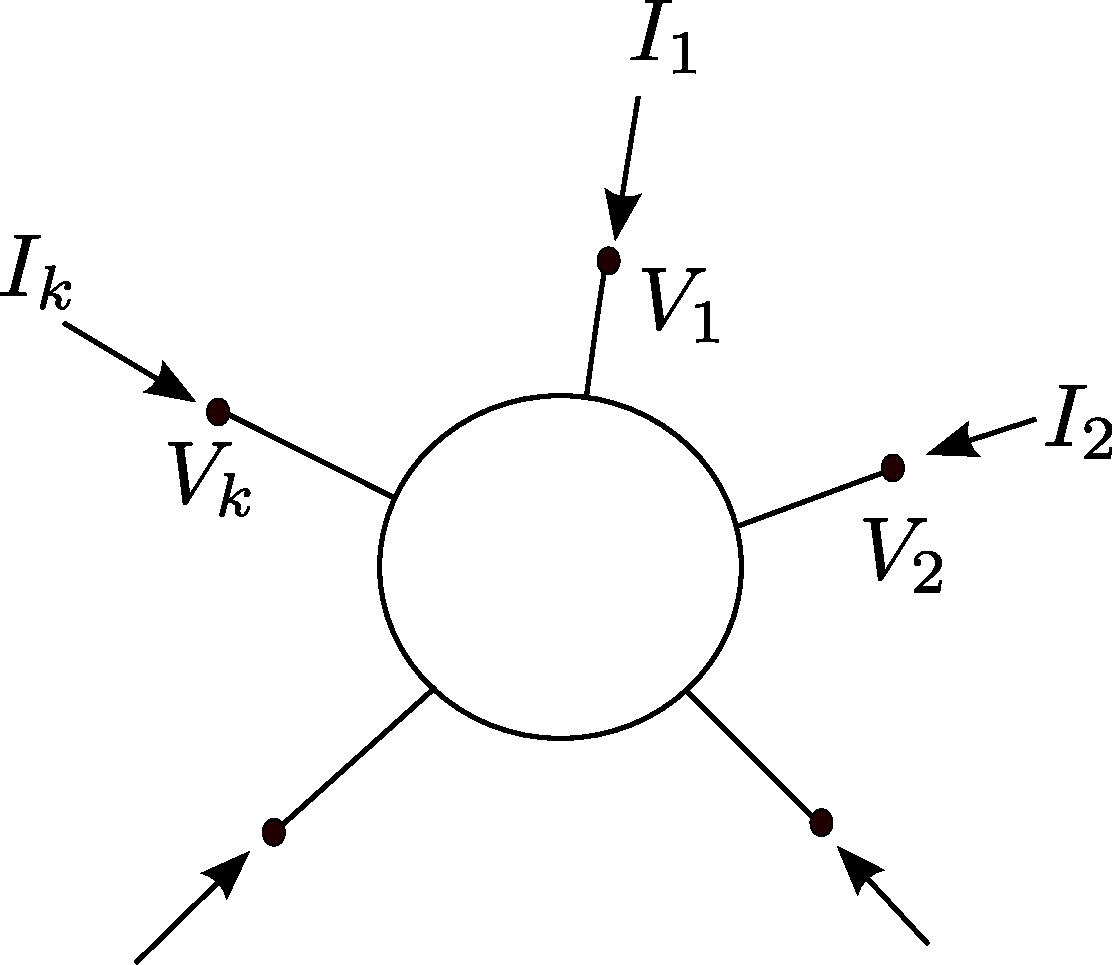
\includegraphics[width=7cm]{systemelec}
\caption{Système électrique}
\label{fig:systemelec}
\end{center}
\end{figure}

Le comportement du système est donné par l'ensemble de toutes les trajectoires $(I_1(t), V_1(t), I_2(t), V_2(t), \ldots, I_k(t), V_k(t))_{t \in \real}$ possibles pour le système. Cet ensemble de trajectoires possède des symétries. En effet, les lois de l'électricité nous enseignent que les potentiels ne sont définis qu'à une constante près. Autrement dit, si $(I_1(t), V_1(t), I_2(t), V_2(t), \ldots, I_k(t), V_k(t))_{t \in \real}$ est une trajectoire possible, alors $(I_1(t), V_1(t)+V, I_2(t), V_2(t)+V, \ldots, I_k(t), V_k(t)+V)_{t \in \real}$ est également une trajectoire possible. De plus, dans la quasi-totalité des circuits réalisés aujourd'hui, il n'y a pas d'accumulation de charge électrique: le système reste neutre électriquement, ce qui implique que $I_1(t) + I_2(t) + \ldots + I_k(t)=0$ à tout instant $t$.

Notons que la puissance transmise au circuit par l'environnement au temps $t$ est $\sum_i V_i(t) I_i(t)$. Cette formule a un sens physique univoque grâce aux deux relations ci-dessus: translater tous les voltages d'une constante ne modifie pas la puissance reçue. 


Les circuits électriques les plus simples ont seulement deux bornes, nommés  pour cela dipôles. Dans ce cas, il suffit de deux variables pour caractériser les trajectoires: la différence de potentiel, ou tension, $v(t)=V_1-V_2$ et le courant $i(t)=I_1(t)=-I_2(t)$ (voir fig.~\ref{fig:dipole}). Les sens du courant et la tension sont choisis de manière conventionnelle.
\begin{figure}[t]
\begin{center}
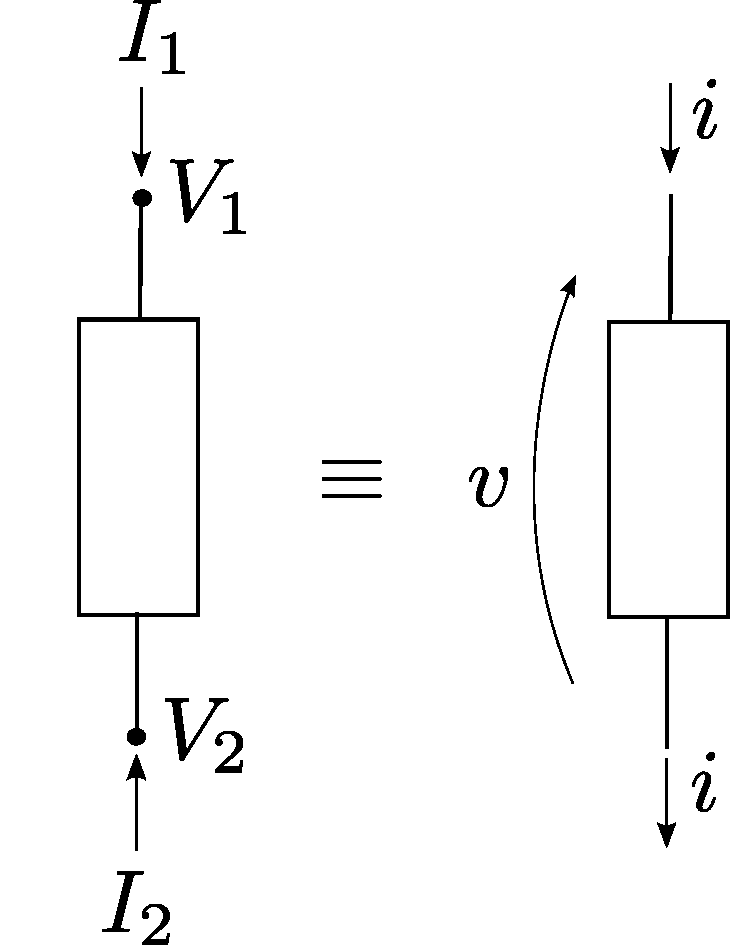
\includegraphics[width=5cm]{dipole2}
\caption{Dipôle électrique}
\label{fig:dipole}
\end{center}
\end{figure}
La tension représente donc l'énergie nécessaire pour déplacer une charge électrique unitaire à travers le dipôle.  On peut également avoir des tripôles (sytèmes à trois bornes, tels que les transistors) ou des quadrupôles (par exemple les transformateurs). 

Dans ce cours, 
nous ne considérons que les circuits dont le comportement 
(l'ensemble des trajectoires possibles) peut être décrit par un modèle d'état 
comme défini au Chapitre 1, où chaque variable extérieure (voltage ou courant) 
est pris, soit comme une entrée $u_i$, soit comme une sortie $y_i$. 
Les variables d'état peuvent être des voltages, courant, flux ou charges,
 comme on le verra. Ce type de modèle d'état cantonné aux équations différentielles est restrictif, en ce qu'il nous interdit par exemple de modéliser commodément les élément de délai, dont le comportement vérifie une équation de délai de type $y(t)=u(t-1)$ (donc non différentielle). 



\section{Dipôles élémentaires}


Nous considérons deux types de dip{ô}les élémentaires:
les impédances et les sources.
\begin{description}
\item{\bf Les impédances}
\begin{enumerate}
\item{\em Les résistances}. Les résistances sont des éléments qui transforment l'énergie électrique en chaleur. Elles sont représentées par
le symbole de la figure \ref{fig:impedances} et sont caractérisées
par une relation algébrique entre la tension $v(t)$ et le courant
$i(t)$ :
\eqnn
r(v(t), i(t)) = 0.
\eeqnn
\begin{figure}[t]
\begin{center}
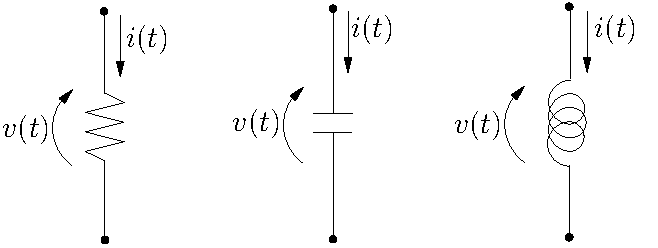
\includegraphics[width=9cm]{impedances}
\caption{Impédances : résistance, capacité, inductance}
\label{fig:impedances}
\end{center}
\end{figure}
Dans le cas d'une résistance linéaire, cette relation se
particularise comme suit (loi d'Ohm) :
\eqnn
v(t) = Ri(t).
\eeqnn
\item {\em Les capacités.} Les capacités sont des éléments qui accumulent les charges électriques. Elles sont représentées par le
symbole de la figure \ref{fig:impedances} et sont caractérisées par la
relation suivante entre la charge $Q(t)$ et le courant $i(t)$ :
\eqnn
i(t) = \frac{dQ(t)}{dt}.
\eeqnn
La charge $Q(t)$ est une fonction de la tension : $Q(v(t))$.  Cette relation peut aussi
s'écrire sous la forme suivante :
\eqnn
i(t) = c(v(t)) \frac{dv(t)}{dt} \;\;
\text{ où } \;\; c(v) \triangleq  \frac{\partial q}{\partial v}.
\eeqnn
Dans le cas d'une capacité linéaire, cette relation se
particu\-larise comme suit :
\eqnn
Q(t) = Cv(t) \;\; \text{ où } \;\; i(t) = C\frac{dv(t)}{dt}.
\eeqnn
\item{\em Les inductances.}  Les inductances sont des éléments qui emmagasinent l'énergie d'un champ magnétique. Elles sont représentées par le
symbole de la figure \ref{fig:impedances} et sont caractérisées, en vertu de
la loi de Faraday, par la relation suivante entre le flux magnétique $\phi(t)$ et la tension
$v(t)$ :
\eqn
v(t) = \frac{d \phi}{dt}. \label{definduc}
\eeqn
On dit que la tension $v(t)$ est {\it induite} par la variation de flux $\phi(t)$ d'où le nom d'inductance. D'une manière générale, cette variation de flux peut être produite par un matériau magnétique en mouvement dans les parages de l'inductance, ou encore par un courant électrique variable circulant dans un conducteur situé à proximité de l'inductance. Dans cette section, nous considérerons uniquement le cas particulier des {\it auto-inductances} où le flux est produit uniquement par le courant traversant le dipôle lui-même. Dans ce cas le flux est une fonction du courant :  $\phi(i(t))$ et la relation (\ref{definduc}) s'écrit aussi sous la forme suivante :
\eqnn
v(t) =  l(i(t)) \frac{di(t)}{dt}
\mbox{ où } l(i) \triangleq  \frac{\partial \phi}{\partial i}.
\eeqnn
Dans le cas d'une (auto)inductance linéaire, cette relation se
particularise comme suit :
\eqnn
\phi(t) = Li(t) \;\; \mbox{ où } v(t) = L \frac{di(t)}{dt}.
\eeqnn
\end{enumerate}
\item{\bf Les sources}
\begin{enumerate}
\item {\em Les sources de tension} représentées par le symbole de
la figure \ref{fig:sources} sont des dip{ô}les définis par la
tension $v(t)$ indépendam\-ment du courant qu'ils débitent.
\begin{figure}[htbp]
\begin{center}
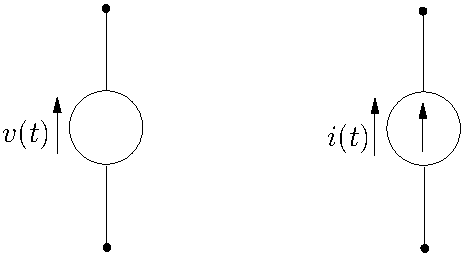
\includegraphics[width=6cm]{sources}
\caption{Sources de tension et de courant}
\label{fig:sources}
\end{center}
\end{figure}
\item{\em Les sources de courant} représentées par le symbole de
la figure \ref{fig:sources} sont des dip{ô}les définis par le
courant $i(t)$ qu'ils débitent indépendamment de la tension à
leurs bornes. 
\end{enumerate} 
\end{description}
Il est important de bien comprendre que les impédances et les sources sont des modèles conceptuels idéaux qui n'ont pas d'existence physique. Les différents éléments dont sont constitués les circuits électriques réels comme par exemple des bobines, des condensateurs ou des batteries sont en pratique modélisés par des assemblages appropriés d'inductances et de sources. Par exemple une source de tension ou de courant est toujours modélisée avec son inévitable résistance interne, comme indiqué sur la fig.~\ref{fig:resint}.

\begin{figure}[t]
\begin{center}
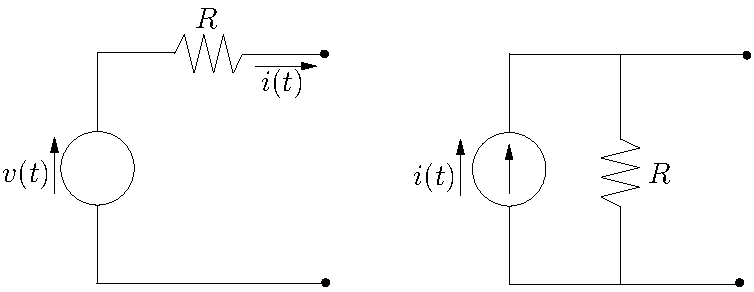
\includegraphics[height=4cm]{resint}
\caption{Sources avec résistances internes}
\label{fig:resint}
\end{center}
\end{figure}


\section{Equivalency between open and closed systems}

We have seen an electrical system as “open”, i.e. equipped with inputs and outputs, which are currents or tensions.  Adding sources, however, allows us to consider an equivalent closed system.  For example, a dipole whose tension $v(t)$ is the input, may be closed by a variable tension source that precisely delivers the tension $v(t)$ (see figure~\ref{fig:equiouvertferme}).  However, for the sake of the analysis, it is comfortable to return to a closed graph.


\begin{figure}[htbp]
\begin{center}
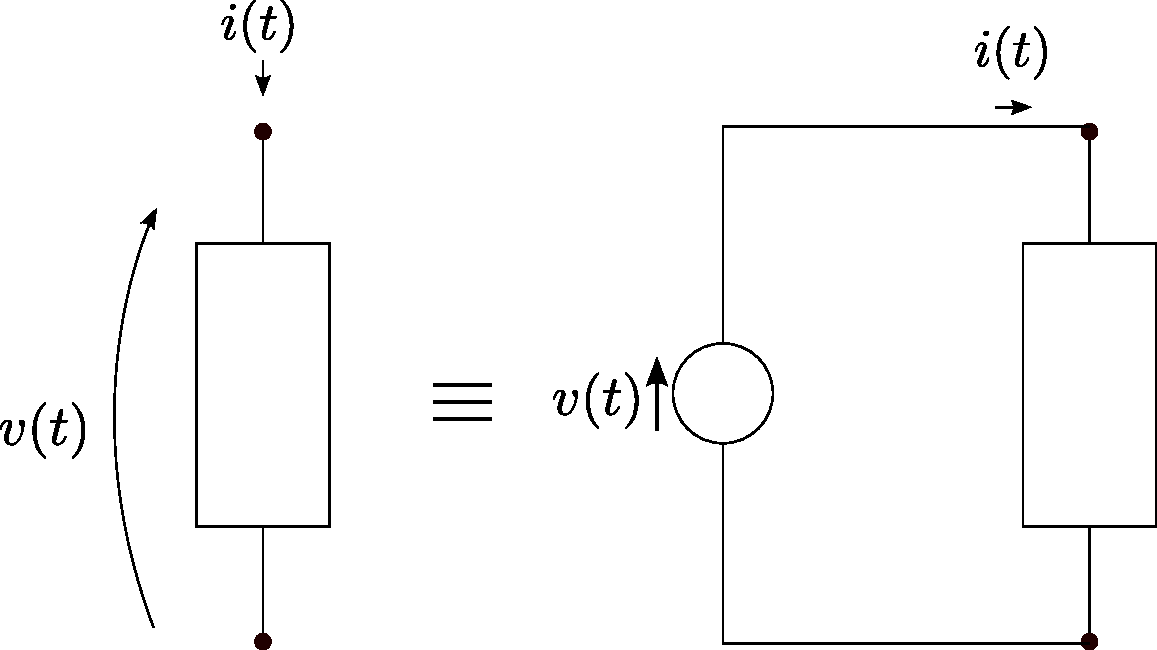
\includegraphics[width=6cm]{equivouvertferme}
\caption{Equivalence between an open circuit and closed circuit:  the case where a dipole where the input is tension and the output power.}
\label{fig:equivouvertferme}
\end{center}
\end{figure}

If the dipole is adapted to supply energy to the outside ($v(t) i(t) >0$), then it can also close the circuit by the load supposed to absorb the energy, often modeled like a (great) load resistance.  For example, an engine is rather of an inductive nature.

\section{Electrical networks and the setting in equation of the state model}

Complex electrical systems are generally created by the interconnection of a defined number of elementary systems.  In this chapter we will consider networks designed by elementary dipoles (impedances and sources)  It is clear that such a network has a graph representation the branches of which are defined by the dipoles.  An example of such a network and its graph is given in figure \ref{fig:exemplereseau}, representing an impedance bridge.  The arrows on the graph indicate the conventional flow chosen by the current in each of the branches.  

\begin{figure}[t]
\begin{center}
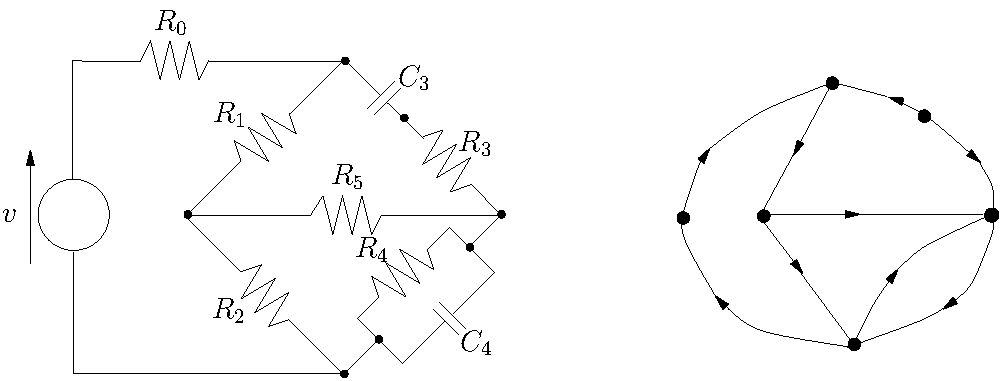
\includegraphics[height=45mm]{exemplereseau}
\caption{Impedance bridge}
\label{fig:exemplereseau}
\end{center}
\end{figure}
We are considering closed associated electrical networks (with sources of tension and/or power, even with load resistors) with $N$ nodes and $M$ branches.  A graph is considered associated when there is link between any two nodes.\\

Let’s define two concepts that will be used subsequently:  meshes and sections of an electrical network.

\begin{description}
\item A {\em mesh} is a cycle, i.e. a closed path without repeating nodes.
\item A {\em section} is an ensemble of branches the extraction of which will split an associated network in at least two associated separate sub-networks.
\end{description}

The organization of a electrical network state model is based on Kirchhoff’s laws, as follows:
\begin{itemize}
\item Kirchhoff’s law on currents:  the algebraic sum of the currents in the branches incident to node a is equal to zero.
\item Kirchhoff’s law on tensions:  the algebraic sum of tensions in a mesh is equal to zero.
\end{itemize}

If the graph is closed, the sum of Kirchhoff’s equations on current of all the $N$ nodes gives the trivial equality $0 = 0$, since each current occurs twice with an opposite sign.  There are $N-1$ Kirchhoff’s independent equations on the currents.  For any section, we also find out that the sum of currents on the brances of the section is equal to zero;  this result is acquired by summing Kirchhoff’s current equations on all nodes on one side of the section.\\

In order to find the number of Kirchhoff’s independent equations on meshes in a closed network, let’s consider the tree at the origin of the graph, i.e. an associated sub-graph, without any mesh or signal breakdown on any of the nodes.  Such a tree has $N - 1$ edges.  Every network branch added to this tree creates one and only one independent mesh.  Thus, we can create $M-N + 1$ mesh equations which will be independent.

Variables of a network state are the currents in some inductors and tensions at the terminals of certain capacitors. In order to establish a state model for a network, we proceed as follows:
\begin{enumerate}
\item Write $N - 1$ Kirchhoff’s equations for all currents
\item Write $M - N +1$ Kirchhoff’s linearly independent equations for all tensions.
\item Write definition impedance laws corresponding to the tensions or currents prevailing in Kirchhoff’s equations.
\item 	Eliminate redundant tensions and currents.
\end{enumerate}

It is interesting to note that if a circuit is comprised of several successive branches creating a dipole composed of several elementary dipoles placed in series, Kirchhoff’s current laws on intermediary nodes will be negligible.  Similarly, Kirchhoff’s mesh equations will only take the total dipole tension into consideration, and not isolated elementary tensions.  As far as writing Kirchhoff’s equations, one can consider this composed dipole as a single branch and two nodes.\\

If the network is comprised of a mesh of capacitors, it is clear that the tension at the terminals of one of those capacitors can be written as the (signed) sum of the others, thus creating a linear relation in state variables.  On the contrary, when a network does not contain a mesh of capacitors, all tensions at the capacitors’ terminals are independent state variables.  Similarly, any inductors section imposes a linear relationship between currents crossing the section, since their (signed) sum is equal to zero.  One of these currents is not considered an independent state variable.  On the contrary, when a network is not comprised of inductors section, all currents in inductors are independent state variables.

\begin{exemple}{\bf \em Rectifier Circuit with Low Pass Filter}

\begin{figure}[htbp]
\begin{center}
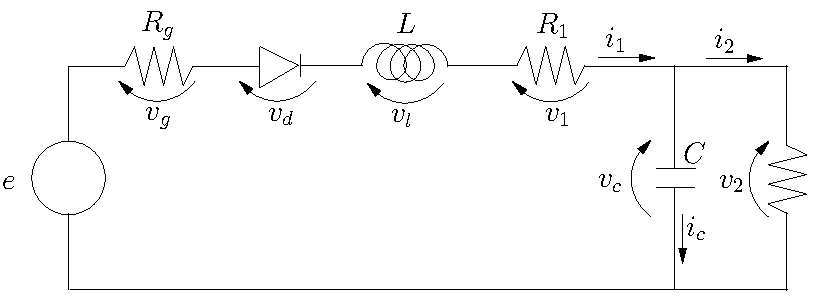
\includegraphics[height=4cm]{redresseur}
\caption{Rectifier Circuit}
\label{fig:redresseur}
\end{center}
\end{figure}

Figure \ref{fig:redresseur} represent a diode rectifier circuit with a filter composed of a capacitor and an inductor.  The diode is a non-linear resistor where the current-tension characteristic is expressed as follows:
\eqnn
i = i_0[e^{\frac{v}{\alpha}} -1]
\eeqnn
where $\alpha$ is a constant proportional to temperature and inversely proportional to the electron charge, whereas $i_0$ defines the leakage current of the diode.  It is clear that the circuit does not contain any capacitors mesh or inductors section. So this state model will have two state variables:  tension $v_c$ at the capacitor terminals et current $i_1$ in the inductor.

The circuit is comprised of $N = 6$ nodes and $M = 7$ branches.  However, for convenience, we can group dipoles in series in one branch which leaves us with $N = 2$ nodes and $M = 3$ branches.  In order to establish the state model of the system, we would then write $N – 1 = 1$ Kirchhoff equation for the currents:
\eqnn
i_c - i_1 + i_2 = 0,
\eeqnn
And $M - N +Where       is self-inductance. In matrix notation that gives 1 =  2$ Kirchhoff equations for the tensions:
\begin{equation} \begin{split}
&v_c - v_2 = 0,\\
&v_g +v_d +v_\ell +v_1 +v_c -e = 0.
\end{split} \end{equation}
These equations are completed by equations of the definition of the different elements of the circuit:
\begin{equation*} \begin{split}
v_g &= R_gi_1, \\
v_d &= \alpha \ln \frac{i_0+i_1}{i_0},\\
v_\ell &= L \frac{di_1}{dt},\\
i_c &= C \frac{dv_c}{dt}, \\
v_1 &= R_1i_1,\\
v_2 &=R_2i_2.
\end{split} \end{equation*}
By eliminating the 7 variables $i_2,i_c, v_g, v_d, v_\ell, v_1, v_2$ between the 9 equations, we easily get the following equations:
\eqnn
&&R_gi_1 + \alpha \ln \frac{i_0+i_1}{i_0} + L \frac{di_1}{dt} + R_1i_1
+ v_c - e = 0,\\
&&C\frac{dv_c}{dt} - i_1 + \frac{v_c}{R_2} = 0.
\eeqnn
By defining the state and input variables as follows:
\e
x_1 = i_1, \;\;\; x_2= v_c, \;\;\; u = e,
\ee
We finally get the following state equations:
\begin{equation*} \begin{split}
\dot x_1 &= -\frac{R_1+R_g}{L} x_1 - \frac{\alpha}{L} \ln
\left(\frac{i_0+x_1}{i_0} \right) - \frac{1}{L} x_2 + \frac{1}{L} u,\\
\dot x_2 &= \frac{1}{C} x_1 - \frac{1}{R_2C} x_2 
\end{split} \end{equation*}
\cqfd

\end{exemple}

When the network contains capacitor meshes or inductor cuts, one searches for a forest (sub-graph without mesh) of maximum size and an inductor non-cut of maximum size.  The number of selected capacitors and inductors represent the number of independent state variables.

%On introduit les définitions
%suivantes :
%\begin{description}
%\item {\em Arbre} : un arbre est un sous-réseau connexe qui contient
%tous les noeuds du réseau mais ne comporte aucune maille (tous les
%arbres d'un réseau ont le même nombre de branches : $N-1$).
%\item {\em Co-arbre}: un co-arbre est le sous réseau
%complémentaire d'un arbre (tous les co-arbres d'un réseau ont le
%même nombre de branches: $M-N+1$).
%\end{description}
%Le nombre de
%variables d'état peut alors être déterminé par la règle suivante :

One can easily demonstrate that is like finding a tree that contains the greatest possible number of capacitors, so that the “co-tree” (i.e. the complementary sub-network of the tree) contains the greatest number of inductors.  The number of independent state variables, thus, is the sum of the number of capacitors and number of inductors of the co-tree.

%L'intuition de cette règle peut se comprendre en observant que les capacités contenues dans un arbre (par définition sans maille) déterminent toutes des variables d'états linéairement indépendantes. On cherchera donc un arbre qui en contiennent le plus grand nombre. De même un coarbre ne contient pas de coupe du réseau. Il est donc avantageux d'y placer un nombre maximal d'inductances, dont les
%courants formeront des variables d'état linéairement indépendantes. Un peu d'algèbre linéaire montre qu'on obtient ainsi un ensemble complet et non redondant de variables d'état. 


\section{Electromechanical systems} 

Could a mechanical system be define similarly with an electric system, whose terminals are subjected, not with currents and voltages, but with forces Fi and speeds $v_i=\dot{q}_i$ (not to be confused with the symbol of tension). Translation all speed $v_i(t)$ vers $v_i(t)+v$ do not modified the behavior of the system, by Galilean relativity. The sum of the forces $\sum_{i} F_i(t)$ in general worthless constantly in the mechanical systems of the engineer. The mechanical energy transmitted to the system under the conditions univocally define as $\sum_i F_i(t) v_i(t)$.  Certain forces or speeds are selected like entries, and others like outputs. An example of a mechanical dipole is a combination of two forces $F_1(t)+F_2(t)=0$ applying to different points  which can be summarized at a couple $T$ and an angular velocity $\omega$! (see Chapter 2)

An electromechanical system is of course defined as a black box whose certain variables are of electric nature and others of mechanical nature (see fig.~\ref{fig:systemelectromec}). 

\begin{figure}[t]
\begin{center}
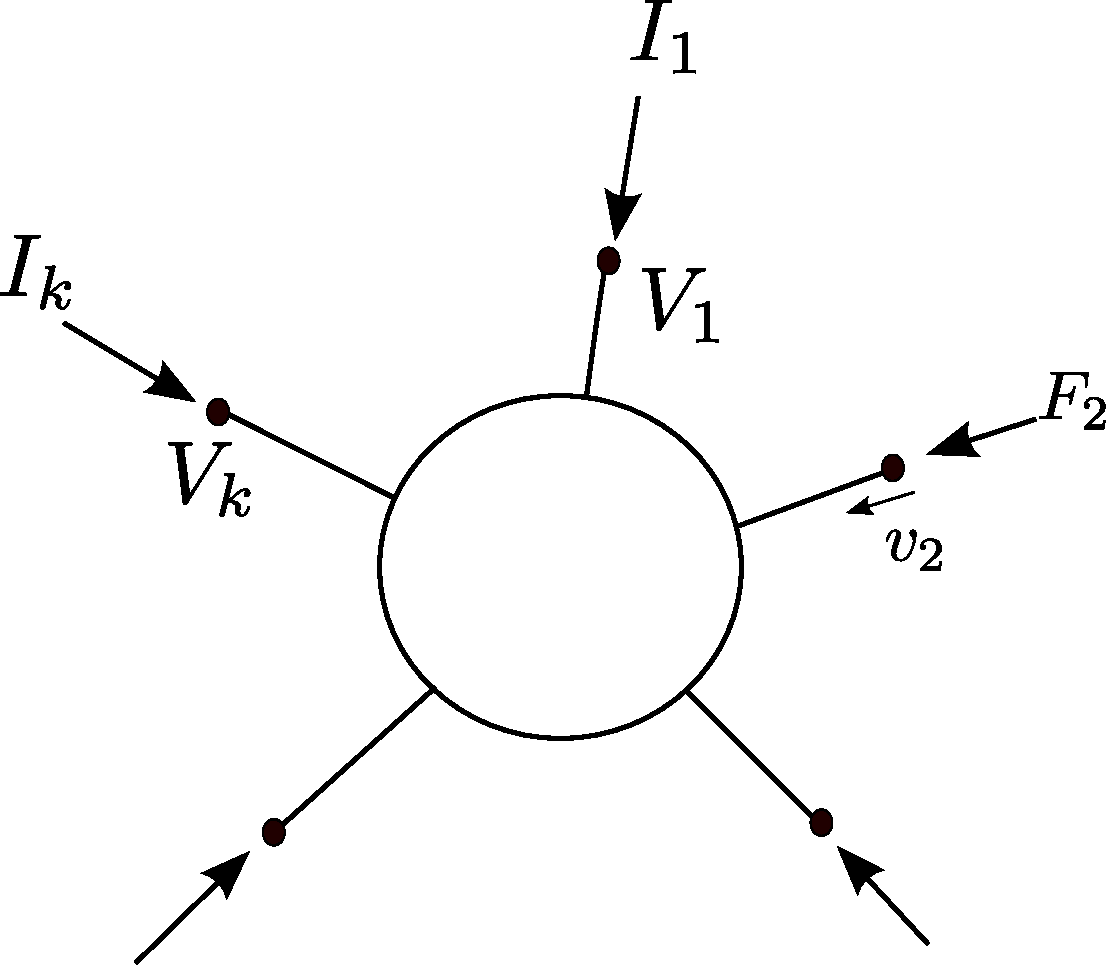
\includegraphics[width=7cm]{systemelectromec}
\caption{Electromechanical system}
\label{fig:systemelectromec}
\end{center}
\end{figure}
For example an electromechanical quadrupole whose variables are $v(t)$, $i(t)$, $T(t)$, $w(t)$ can model a generator if $T\omega<0, vi>0$ electrical energy converted into mechanical energy) or an engine si $T\omega>0, vi<0$ (mechanical energy converted into electrical energy).


\begin{figure}[t]
\begin{center}
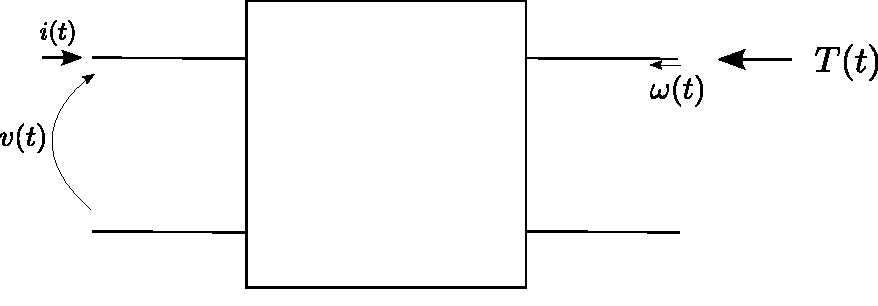
\includegraphics[width=7cm]{quadrupelectromec}
\caption{Electromechanical quadrupole}
\label{fig:quadrupelectromec}
\end{center}
\end{figure}

Concretely, an electromechanical system often arises as an articulated mechanical system (with $p$ degrees of freedom) which can be built partially in a magnetic material and whose certain bodies carry one or more inductive electrical circuits (coils, winding, ...). The equations constitutive of an electromechanical system consequently comprise a mecanical part and an electric part. The two sections that follow explain, with some electromagnetism refreshers, how the electromagnetic variables (loads, flow, currents, tensions) and mechanics (generalized positions, speeds, forces) can interact.

\section{Influence of a mechanical movement on the electric quantities} 

The Faraday’s law $E_i=\frac{d\phi_i}{dt}$ describes the electromotive force (tension) undergone by an inductance crossed by one magnetic flow $\phi_i$. Up to now it was supposed that this flow was created only by the current $I_i$ going through it (self-inductance). For a linear relation  $\phi_i=L_iI_i$, one obtains the law constitutive $V_i=L_i \dot{I}_i$.

Actually each current  $I_j$ generates a magnetic field and thus a flow in the inductance $i$. This flow depends on $I_j$, but also on the relative position of the conductors which carry these currents, possibly varying with time because of the mechanical movement of the parts which support the conductors. Generally only the currents which cross an inductance generate a non-negligeable magnetic field. If $\phi_i$ depends linearly of each $I_j$, one can write
\begin{equation}
\phi_i=\sum_j L_{ij} I_j,
\label{eq:PhiLI}
\end{equation}
Where   $L_{ii}$    is self-inductance. In matrix notation that gives
\begin{equation}
\Phi=L(q) I,
\label{eq:PhiLI2}
\end{equation}
where $L(q)$ is a symmetrical matrix of inductance depending on the generalized positions of the mechanical part $q$. By combining this with the equation of Faraday for each inductance, one arrives at the equations of state
\begin{equation}
E=\sum_k \frac{\partial L}{\partial q_k} \dot{q}_k I + L\dot{I},
\label{eq:VqI}
\end{equation}
which mix positions, speeds, currents and tensions.

The electric component of the electromechanical systems discussed in this chapter are often simply reduced to a set of inductances, each one in  series with a resistance representing inevitable internal resistance or one  resistance of load, which represents the useful consumption of electrical energy possibly generated by the system (see G. 3.11). In this case, voltage at the terminals of the circuits are written in a matrix way
\eqn
V = RI + E \label{ELECM}
\eeqn
where $R$ is the diagonal matrix $\mbox{diag}\{R_i, i = 1,m\}$ and the vectors  $V,I$ and $E$ are defined as follows:
\begin{equation*} \begin{split}
V^T &= (v_1, v_2, \ldots, v_m),\\
I^T &= (I_1, I_2, \ldots, I_m),\\
E^T &= (E_1, E_2, \ldots, E_m).
\end{split} \end{equation*}
\begin{figure}[t]
\begin{center}
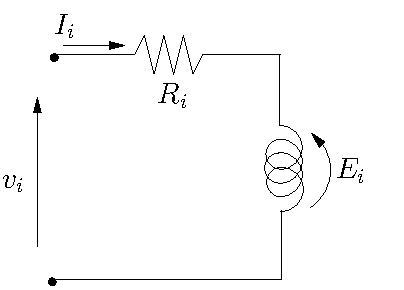
\includegraphics[height=4cm]{circel}
\caption{Basic circuit}
\label{fig:circel}
\end{center}
\end{figure}

\section{Creation of a mechanical movement by electromagnetic fields} 

A magnetic field exerts a force known as Force of Lorentz on each carrier of moving load. By integrating this force on all the charge carriers set in movement by an electric current in a conductor one obtains a macroscopic force, known as Laplace force.


%Pour peu que ce conducteur appartienne à une boucle rectangulaire de dimension $l \times z$ et soit mobile dans la direction de $z$ (voir Fig.~\ref{fig:laplace}, on constate que cette force de Laplace est aussi proportionnelle à $\frac{\partial \phi}{\partial z}I$,
%où $\phi$ est le flux créé par $B$ dans la boucle traversée par le courant $I$. 

%\begin{figure}[t]
%\begin{center}
%\includegraphics[width=7cm]{laplace}
%\caption{Force de Laplace sur un conducteur mobile posé sur deux rails conducteur}
%\label{fig:laplace}
%\end{center}
%\end{figure}

In general, one can show that the Laplace force on the coordinate $q_k$ is
\begin{equation}
F_k=\frac{1}{2}\sum_i \frac{\partial \phi_i}{\partial q_k}  I_i = \frac{1}{2} I^T \frac{\partial L}{\partial q_k} I,
\label{eq:Lorentz}
\end{equation}

the last equality concerning linear inductances.  In the latter case case, one can directly assume the expression $F_k$ supposing that the force originates from a potential energy contained in inductances which generate the magnetic fields,
expressed by $\frac{1}{2} I^T L(q_k) I$.




%\begin{description}
%\item{\em Equations mécaniques}.  Les équations
%de la partie mécanique prennent la forme générale que nous avons
%obtenue au chapitre 2.
%\eqn
%M(q) \ddot q + F(q, \dot q) = G_{em}(q) u_{em} + G_a(q)u_a.
%\label{EMECA}
%\eeqn
%Dans cette équation, $u_{em}$ représente les forces
%généralisées d'origine électromagnétique (équation de Lorentz)
%tandis que $u_a$ désigne les autres forces généralisées qui
%s'appliquent éventuellement au système. $q$ est un vecteur de dimension $p$.
%\item {\em Equations électriques}.  Chacun des circuits électriques
%du système peut être conceptualisé par le circuit
%élémentaire représenté sur la fig \ref{fig:circel} où
%$R_i$ représente la résistance propre du circuit et $E_i$
%représente la tension induite par les variations de flux magnétiques produits par les différents
%circuits (y compris l'auto-induction) et par le mouvement du système
%(loi d'induction électromagnétique ou loi de Lenz). 
%\begin{figure}[t]
%\begin{center}
%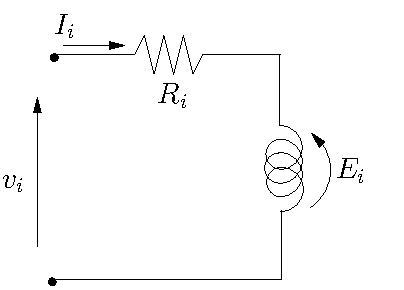
\includegraphics[height=4cm]{circel}
%\caption{Circuit élémentaire}
%\label{fig:circel}
%\end{center}
%\end{figure}
%Si l'on
%suppose que le système comporte $m$ circuits, on obtient
%un ensemble d'équations de Kirchhoff de la forme
%\eqnn
%R_i I_i +E_i = v_i, \;\;\;   i = 1, \ldots, m.
%\eeqnn
%Dans ces équations, $v_i$ représente la tension aux bornes du
%dip{ô}le équivalent du réseau connecté au circuit.  Le plus
%souvent, il s'agit simplement soit d'une source de tension ou de
%courant, soit d'une impédance de charge.  L'ensemble des équations
%électriques peut aussi s'écrire sous forme matricielle
%\eqn
%V = RI + E \label{ELECM}
%\eeqn
%où $R$ est la matrice $\mbox{diag}\{R_i, i = 1,m\}$ et les
%vecteurs $V,I$ et $E$ sont définis comme suit :
%\begin{equation*} \begin{split}
%V^T &= (v_1, v_2, \ldots, v_m),\\
%I^T &= (I_1, I_2, \ldots, I_m),\\
%E^T &= (E_1, E_2, \ldots, E_m).
%\end{split} \end{equation*}
%\end{description}
%La mise en équation complète du modèle d'état d'un système
%électro\-mécanique particulier requiert l'explicitation des
%{\em couplages} entre la partie mécanique (\ref{EMECA}) et
%la partie électrique (\ref{ELECM}), c'est à dire l'expression des
%forces généralisées électromagnétiques $u_{em}$ d'une part et
%des tensions induites $E$ d'autre part comme des
%fonctions des coordonnées mécaniques $q, \dot q$ et des courants
%électriques $I$~:
%\eqnn
%u_{em}(q, \dot q, I), \hspace{1cm} E(q,\dot q, I). 
%\eeqnn 
%Chacune des tensions $E_i$ peut se décomposer comme
%suit~:
%\eqn \label{ei}
%E_i = \sum^m_{j=1} e_{ji} 
%\eeqn
%où $e_{ji}$ représente la tension induite par le circuit $j$ sur le
%circuit $i$ (en particulier, $e_{ii}$ représente l'auto-induction
%du circuit $i$). Par application de la loi de Faraday, chacune de ces tensions
%s'exprime comme suit :
%\eqnn
%e_{ji} = \frac{d\phi_{ji}}{dt}
%\eeqnn
%où $\phi_{ji}$ est le flux induit par le circuit $j$ sur le circuit
%$i$.
%Le flux $\phi_{ji}$ varie en fonction du courant $I_j$ dans le
%circuit inducteur et de la position $q$ du système :
%\eqnn
%\phi_{ji} = \varphi_{ji}(q, I_j).
%\eeqnn
%On en déduit que la tension $e_{ji}$ s'écrit :
%\eqn \label{eij}
%e_{ji} = \frac{\partial \varphi_{ji}}{\partial q} \dot q +
%\frac{\partial \varphi_{ji}}{\partial I_j} \dot I_j.
%\eeqn
%D'autre part, la composante d'indice $k$ du vecteur
%des forces généralisées $u_{em}$ s'écrit 
%\eqn
%u_{em(k)} = \frac{1}{2} \sum^m_{i=1} \sum^m_{j=1} \frac{\partial
%\varphi_{ji}}{\partial q_k} I_i. \label{uem}
%\eeqn
%Finalement, en combinant les équations (\ref{EMECA}),(\ref{ELECM}),
%(\ref{ei}), (\ref{eij}), (\ref{uem}), on obtient un modèle d'état
%comportant $2p + m$ variables d'état $q, \dot q, I$.

\vspace{2mm}
\begin{exemple}{\bf \em  An electromechanical system of positioning.} 
 
The flow diagram of an electromagnet used for a positioning of precision is indicated in figure \ref{fig:relaisem}.
\begin{figure}[htbp]
\begin{center}
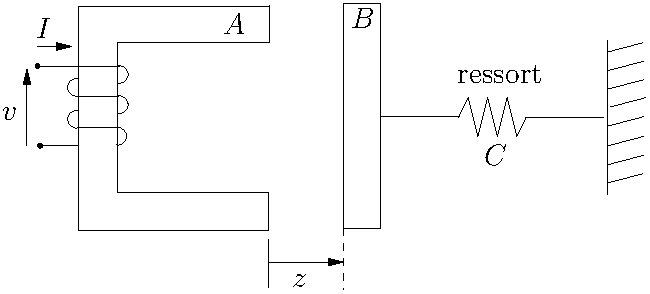
\includegraphics[height=4cm]{relaisem}
\caption{An electromechanical system of positioning}
\label{fig:relaisem}
\end{center}
\end{figure}
The electromagnet $A$ is equipped with an inductor coil in which circulates an inductor current $I$. The metal piece $B$ is mobile and subject to a linear traction force by the spring $C$  

The magnetic flow varies proportionally with the current $I$ and inversely proportionally to the distance $z$ in the gap between $A$ and $B$.
\eqnn
\phi (I,z) = \frac{\alpha I}{1+\beta z}.
\eeqnn
This is an instance of the magnetic law of Ohm (or law d’Hopkinson) which expresses the magnetic flow (equivalent of the current flow of electric charges) like the ratio between the magnetomotive flow (proportional of the current) and the reluctance (resistance of material to the magnetic flow) which is proportional to the length of the circuit.

The tension inducted in the circuit is thus written :
\eqnn
e &=& \frac{d\phi}{dt} = \frac{\partial \phi}{\partial I}
\frac{dI}{dt} + \frac{\partial \phi}{\partial z} \frac{dz}{dt}\\
&=&\frac{\alpha}{1+\beta z} \frac{dI}{dt} - \frac{\alpha \beta
I}{(1+\beta z)^2} \frac{dz}{dt}.
\eeqnn
The electromagnetic force of origin being exerted on the moving part is written :
\eqnn
F_{em} = \frac{1}{2} I \frac{\partial \phi}{\partial z} = -
\frac{\alpha \beta}{2} \left(\frac{I}{1+\beta z}\right )^2.
\eeqnn
In agreement with the physical intuition, one observes that this force tends to bring closer the part $B$ to the electromagnet whatever the direction of the courant $I$.
One can then write the dynamic equations of the system. \\

\begin{itemize}
\item{\em Mechanic equation}
\begin{eqnarray}
m \ddot z &=& k(z_o - z) + F_{em}\\
&=& k(z_o - z) - \frac{\alpha \beta}{2} \left (\frac{I}{1+\beta z}
\right )^2
\end{eqnarray}
where $m$ indicates the mass of the constant part $B$, $k$ the contant of the rearward movement of the $s_0$ spring and the position of the spring at rest\\
\item{\em Electric equation}
\begin{eqnarray}
V&=& RI + e\\
  &=& RI + \frac{\alpha}{1+\beta z} \dot I - \frac{\alpha \beta I}{(1+
\beta z)^2} \dot z 
\end{eqnarray}
where $R$ indicated the resistance of the electric circuit. 
\end{itemize}

By introducing the following definitions of the state variables
\eqnn
x_1 = z, \;\;\; x_2 = \dot z, \;\;\; x_3 = I
\eeqnn
and of the variable of entry:
\eqnn
u = V,
\eeqnn
Finally:
\begin{eqnarray}
\dot x_1 &=& x_2,\\
\dot x_2 &=& \frac{k}{m}(z_o - x_1) - \frac{\alpha \beta}{2m} \left
(\frac{x_3}{1+ \beta x_1} \right )^2,\\
\dot x_3 &=& \frac{\beta x_2 x_3}{1+\beta x_1} - \frac{R}{\alpha}(1+
\beta x_1) x_3 + \frac{1 + \beta x_1}{\alpha} u.
\end{eqnarray}
\cqfd

\end{exemple}

\section{Rotating electric machines}

The rotating electric machines constitute a particular category of electromechanical systems formed by two bodies. The first one, called {\em rotor}, is in rotation around an axe whose position is fixed to the second one, called {\em stator}. These two pieces are provided with different \blue {field windings} whose utility is to realise electromechanical conversions of which the machines are the centre. 

When the stator itself is fixed to the inertial landmark, an electrical machine has only one mechanical degree of freedom : the rotor’s rotation angle, written $\theta$. The mechanical part of the system shrinks therefore to a scalar equation of the form : 

\eqn \label{meca}
J \ddot \theta + h(\dot \theta) = T_{em}+ T_a 
\eeqn
where $h(\dot \theta)$ represents the friction torque, $T_{em}$ the electromagnetical torque and $T_a$ all the other external torques applied to the rotor. 

On the other hand, the electrical part of the dynamic has the general form (\ref{ELECM}) :
\eqnn
V = RI + E. 
\eeqnn

In most running machines, when the magnetical saturation effects are negligible (or neglected), it is possible to present the flows $\phi_{ij}$ by an expression of the form : 

\eqnn
\phi_{ij} = L_{ij}(\theta)I_i
\eeqnn
which is linear to the inductor current $I_i$ but that depends on the angular position $\theta$ of the rotor, following a law $L_{ij}(\theta)$ usually periodic. The inductance matrix (symmetrical) is defined as : 

\eqnn
L(\theta) \triangleq [L_{ij}(\theta)]
\eeqnn
and its derivative to $\theta$ is : 
\eqnn
K(\theta) \triangleq \frac{\partial L(\theta)}{\partial \theta}.
\eeqnn
Then, the use of the theory that was introduced in the last sections leads to general equations of electromechanical coupling, whose form is the following: 
\begin{align}
E &= L(\theta)\frac{dI}{dt} + \frac{d\theta}{dt}K(\theta)I, \label{coup1}\\
T_{em} &= \frac{1}{2}I^TK(\theta)I. \label{coup2}
\end{align}
By combining the equations (\ref{meca}),(\ref{ELECM}),(\ref{coup1}) and (\ref{coup2}) we get the general model of the electrical machines~: 
\begin{equation*} \begin{split}
L(\theta)\dot I &= - \omega K(\theta) I - RI + V, \\
\dot \theta &= \omega, \\
J \dot \omega &= \frac{1}{2} I^TK(\theta)I - h(\omega) + T_a.
\end{split} \end{equation*}
It is this general model that is on the basis of the particular models establishment in the applications. Often, but it not a standard, the voltage vector $V$ or the torque $T_a$ are parameterized by  well selected entrance variables that represent the external influence on the machine’s behaviour. Here is an example. Other examples are provided in the exercises. 

\begin{exemple}{\bf \em Elementary machine with two windings}

Let’s consider an electrical machine whose rotor and stator are concentric cylinders with a winding on the stator and another on the rotor ( Fig.~\ref{fig:rotorstator}). The statorical and rotorical auto-inductances $L_s$ and $L_r$ are constants. The mutual inductance $L_{sr}$ is a cosinusoidal periodical function of angle $\theta$  

\eqnn
L_{sr}(\theta) = L_o \cos \theta.
\eeqnn

Matrices $L(\theta)$ and $K(\theta)$ are written as follows:

\eqnn
L(\theta) =   \bma{cc} L_s & L_o \cos \theta\\ L_o \cos \theta & L_r \ema
\;\;\;\;  K(\theta) = \bma{cc} 0 & -L_o \sin \theta\\ -L_o \sin \theta & 0
\ema.
\eeqnn
Vectors of current and induced tensions are noted : 
\eqnn
I = \bma{c} I_s \\ I_r \ema \;\;\;\; E = \bma{c} e_s \\ e_r \ema.
\eeqnn
Electromechanical coupling equations (\ref{coup1}), (\ref{coup2})  particularize themselves by:
\begin{equation*} \begin{split}
e_s &= L_s \dot I_s + L_o \cos\theta \dot I_r - \dot \theta L_o \sin \theta
I_r, \\ 
e_r &= L_r \dot I_r + L_o \cos\theta \dot I_s - \dot \theta L_o \sin
\theta I_s, \\
T_{em} &= -L_o \sin \theta I_sI_r.
\end{split} \end{equation*}
The rotorical circuit is being supplied by a constant current source $I_r$. Such a machine can be used either as a generator (that transforms the mechanical power provided by the external torque $T_a$ in electrical power delivered by the statoric electromotive power $e_s$), or as an engine  (that transforms the electrical power delivered to the stator by the source $v_s$  in a mechanical power delivered by the electromagnetical torque $T_{em}$). 

\begin{figure}[htbp]
\begin{center}
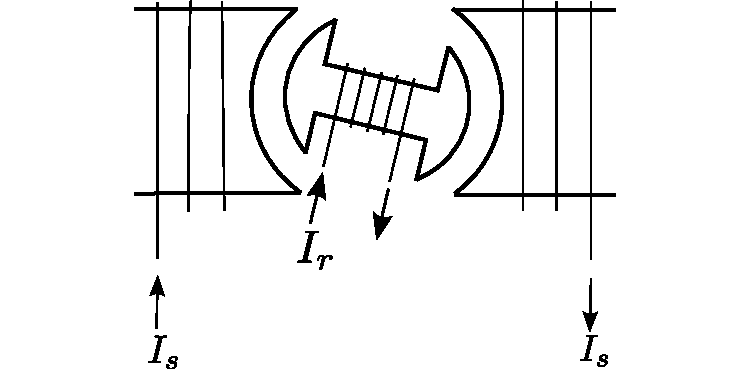
\includegraphics[height=5cm]{rotorstator}
\caption{Elementary machine with two windings}
\label{fig:rotorstator}
\end{center}
\end{figure}

The system has three state variables :
\begin{equation*} \begin{split}
x_1 &= I_s, \\
x_2 &= \theta, \\
x_3 &= \dot \theta,
\end{split} \end{equation*}
and two input variables :
\begin{equation*} \begin{split}
u_1 &= v_s, \\
u_2 &= T_a.
\end{split} \end{equation*}
The state-spaced model of the system is noted as follows: 
\begin{align*}
L_s\dot x_1 &= L_oI_rx_3 \sin x_2 - R_s x_1 + u_1, \\
\dot x_2 &= x_3, \\
J\dot x_3 &= -h(x_3) - L_oI_rx_1 \sin x_2 + u_2.
\end{align*}

In the case of generator mode, we can also close the electrical part of the circuit with a resistance of charge $R_L$, we can then set $u_1=R_L x$ and we obtain a state-spaced model with only one input $u_2=T_a$.

\cqfd



\end{exemple}

\section{Direct current machines}
\markboth{{\hspace*{5mm}\bf Chapitre 3} \hfill Electrcical systems}{{ \bf Sec. \thesection}
\hfill Direct current machines\hspace*{5mm}} 


Direct current machines (fig.
\ref{fig:machineDC}) generally include a stator winding and a rotor one.  
\begin{figure}[t]
\begin{center}
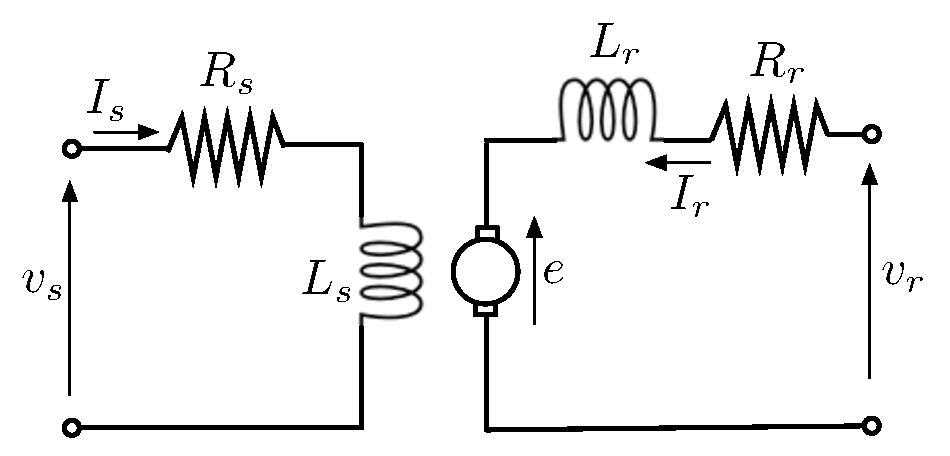
\includegraphics[height=4cm]{machineDC}
\caption{Direct current machines}
\label{fig:machineDC}
\end{center}
\end{figure}

The stator winding is the inductive circuit whose current is noted  by $I_s$. The rotor winding is the \blue {induced circuit} whose current is written by $I_r$. 

So a direct current machine (DC machine) seems similar to the elementary two-winding machine we studied in the previous section. However, there is a fundamental difference : a DC machine is designed with a 
\blue {commutation} system whose effect is to modify the electromechanical coupling. A detailed description of this commutation effect on the coupling equations is beyond the scope of this book.  So we restrict ourselves to give the results. When the effect of magnetic saturation are negligible and when the commutation  
doesn't generate significant non-linearities, the equations  of electromechanical coupling  of a DC machine are witten  as the following multilinear form :
 
\begin{equation*} \begin{split}
&e_s = L_s \frac{dI_s}{dt}, \\[2mm]
&e_r = L_r \frac{dI_r}{dt} + \frac{d\theta}{dt}K_eI_s, \\[2mm]
&T_{em} = K_mI_rI_s.
\end{split} \end{equation*}
Let's notice the the \blue {resemblance, but not the similarity},
of those equations with the general one (\ref{coup1}), (\ref{coup2}) of electrical machines without commutation which have been previously defined. We notice in particular the default of symmetry between 
the form of $e_s$ and the one of $e_r$ which is precisely  due to commutation. 

According to the way they are build and implemented, direct current machines can be used as motors or as generators.
Here are some usual examples of applications. \\

\noindent{\em General model for DC machine}

The system has four state variables  :
\begin{equation*} \begin{split}
x_1 &= \theta, \\
x_2 &= \dot{\theta}, \\
x_3 &= I_s, \\
x_4 &= I_r.
\end{split} \end{equation*}
The system inputs are the voltages at the terminals of the inductor circuit $v_s$ and of the induced circuit $v_r$ as well as  the external torque $T_a$ :
\begin{equation*} \begin{split}
u_1 &= v_s, \\
u_2 &= v_r, \\
u_3 &= T_a.
\end{split} \end{equation*}
The state-spaced model can be written as follows :
\begin{equation*} \begin{split}
\dot x_1 &= x_2,\\
J\dot x_2 &= -h(x_2) + K_m x_3x_4 + u_3,\\
L_s\dot x_3 &= -R_s x_3 + u_1,\\
L_r\dot x_4 &= -R_r x_4 - K_ex_2x_3 + u_2.
\end{split} \end{equation*}
\\
\noindent{\em DC engine controlled by stator.}

It's a DC engine whose rotor current is provided by a constant current source (figure \ref{fig:cominducteur}) :
\eqnn
I_r = constant
\eeqnn
\begin{figure}[htbp]
\begin{center}
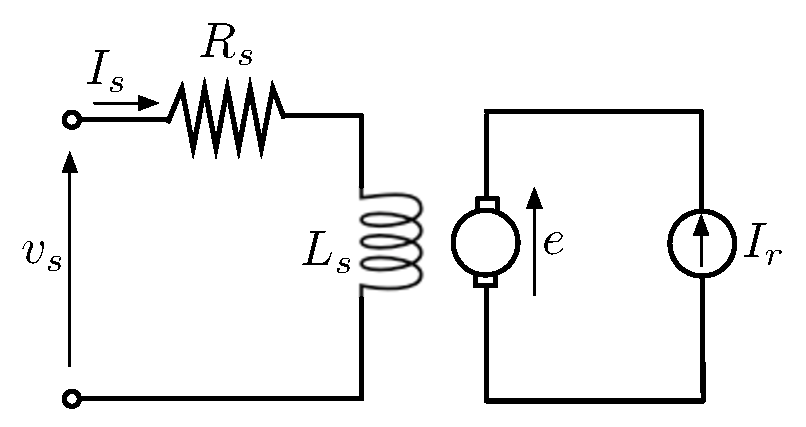
\includegraphics[height=4cm]{cominducteur}
\caption{ DC engine controlled by the stator}
\label{fig:cominducteur}
\end{center}
\end{figure}

\noindent The system has three state variables :
\begin{equation*} \begin{split}
x_1 &= \theta, \\
x_2 &= \dot{\theta}, \\
x_3 &= I_s. 
\end{split} \end{equation*}
The system inputs are the voltages at the terminals of the stator circuit $v_s$ and the external torque $T_a$ : 
\begin{equation*} \begin{split}
u_1 &= v_s, \\
u_2 &= T_a.
\end{split} \end{equation*}
The state-spaced model is written as follows :
\begin{equation*} \begin{split}
\dot x_1 &= x_2,\\
J\dot x_2 &= -h(x_2) + K_m I_r x_3 + u_2,\\
L_s\dot x_3 &= -R_s x_3 +u_1.
\end{split} \end{equation*}
\\
\noindent{\em DC engine controlled by the rotor.}

It's a DC engine whose stator current is provided by a constant current source ( figure \ref{fig:cominduit}):
\eqnn
I_s = constant
\eeqnn
\begin{figure}[htbp]
\begin{center}
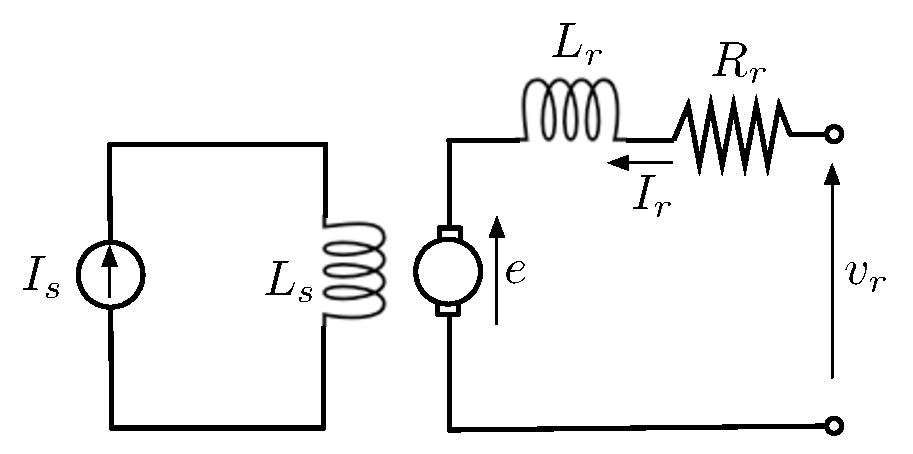
\includegraphics[height=4cm]{cominduit}
\caption{DC engine controlled by rotor}
\label{fig:cominduit}
\end{center}
\end{figure}
The system has three state variables :
\begin{equation*} \begin{split}
x_1 &= \theta, \\
x_2 &= \dot{\theta}, \\
x_3 &= I_r. 
\end{split} \end{equation*}
The system inputs are the voltage at the terminals of the rotor circuit $v_r$ and the external torque $T_a$ : 
\begin{equation*} \begin{split}
u_1 &= v_r, \\
u_2 &= T_a.
\end{split} \end{equation*}
The state-spaced model is written as follows :
\begin{equation*} \begin{split}
\dot x_1 &= x_2,\\
J\dot x_2 &= -h(x_2) + K_m I_s x_3 + u_2,\\
L_r\dot x_3 &= -R_r x_3 - K_e I_s x_2 + u_1.
\end{split} \end{equation*}
\\
\noindent{\em DC generator.}
The function of a generator is to convert mechanical power in electrical power \blue{delivered} by the rotor circuit on any load impedance of $Z_L$.

When this impedance is resistive ($R_L$),  the system has three state variables ( figure
\ref{fig:genDC})~: 
\begin{equation*} \begin{split} 
x_1 &= I_s, \\ x_2 &= I_r, \\ x_3 &= \omega.
\end{split} \end{equation*}
\begin{figure}[htbp]
\begin{center}
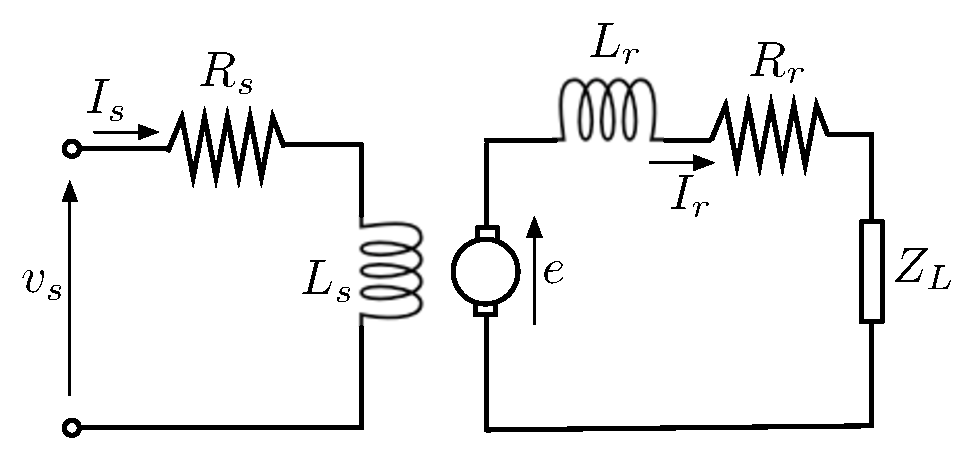
\includegraphics[height=4cm]{genDC}
\caption{ DC generator}
\label{fig:genDC}
\end{center}
\end{figure}
The system inputs are the voltage at the terminals of the stator circuit $v_s$ and the torque $T_a$ :
\begin{equation*} \begin{split}
u_1 &= v_s, \\
u_2 &= T_a.
\end{split} \end{equation*}
The state-spaced model is written as follows :
\begin{equation*} \begin{split}
L_s\dot x_1 &= -R_s x_1+ u_1, \\
L_r\dot x_2 &=  - (R_r +R_L) x_2 - K_e x_3 x_1,\\
J\dot x_3 &= -h(x_3) + K_m x_1x_2 + u_2.
\end{split} \end{equation*}


\section{Exercices}

\begin{exercice} {\bf \em Linear circuit}

Establish a state-spaced model of the linear circuit shown in figure  \ref{fig:circuitlin} with the applied voltage $e$ and the adjustable resistance $r$ as input variables. \qed
 \begin{figure}[htbp]
\begin{center}
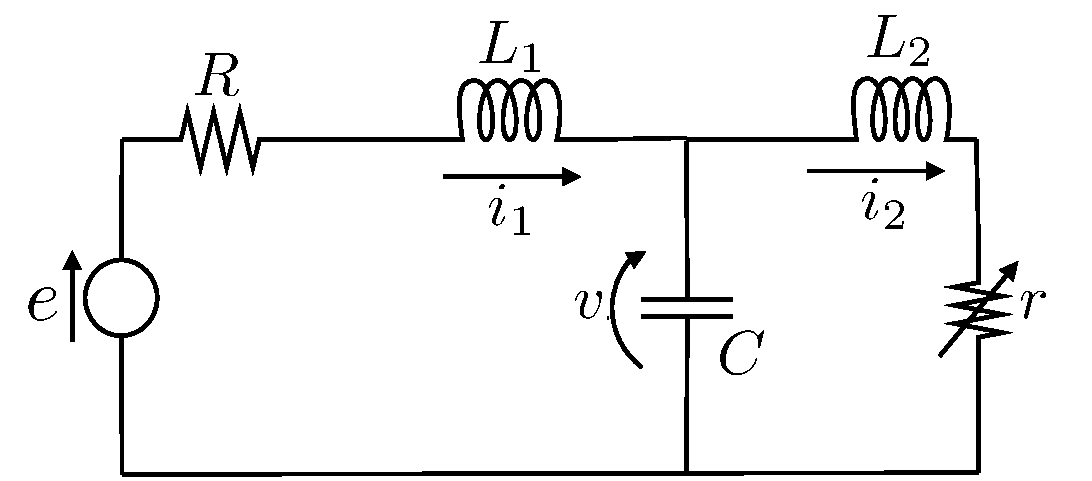
\includegraphics[height=4cm]{circuitlin}
\caption{Linear circuit}
\label{fig:circuitlin}
\end{center}
\end{figure}

\end{exercice}
\vv

\begin{exercice} {\bf \em Voltage doubler bridge}

The electrical diagram of a voltage doubler bridge is shown in figure \ref{fig:pont}. Establish the state-spaced model of the system assuming that all the dipoles are linear except the diodes. \qed
\begin{figure}[htbp]
\begin{center}
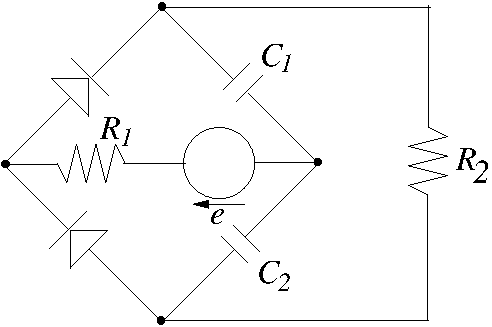
\includegraphics[height=4cm]{pont}
\caption{Voltage doubler bridge}
\label{fig:pont}
\end{center}
\end{figure}
\end{exercice}
\vv

\begin{exercice} {\bf \em Transformer}
The electrical diagram of a transformer is shown in figure
\ref{fig:transfo}.
\begin{figure}[htbp]
\begin{center}
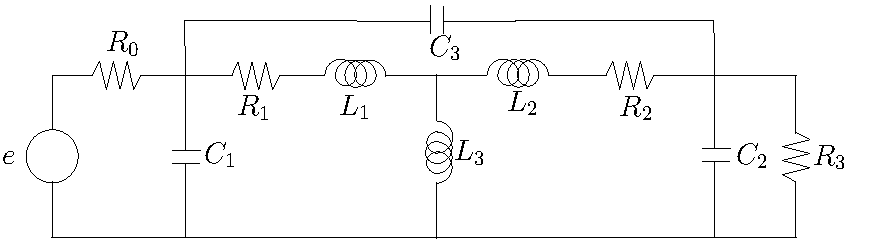
\includegraphics[height=3cm]{transfo}
\caption{Transformer equivalent circuit}
\label{fig:transfo}
\end{center}
\end{figure}
\begin{enumerate}
\item Has this electrical network some capacity \blue {mesh} and/or inductance \blue {cuts} ? 
 Explain your answer.
\item Establish the state-spaced model assuming that the dipoles are linear. \qed
\end{enumerate}
\end{exercice}
\vv

\begin{exercice}{\bf \em  A circuit with a tunnel diode}

A electrical circuit is described by the following state equations :
\eqnn
C \dot x_1 &=& -h(x_1)+x_2,\\
L\dot x_2 &=& -x_1-Rx_2 +u.
\eeqnn
$x_1$ is the voltage to the terminals of a linear capacity, $x_2$ is the current in a linear inductance, $h(x_1) = x^3_1 - 10 x^2_1 + 25 x_1$  
is the characteristic of a tunnel diode. Establish the circuit diagram. \qed
\end{exercice}
\vv

\begin{exercice}{\bf \em Electromechanical converter }

The device illustrated in figure \ref{fig:convem} transforms an electrical power provided
by the voltage source in a mechanical mouvement of translation.  It is made of a cylindrical steel core moving
longitudinally inside a solenoid. \qed
\begin{figure}[htbp]
\begin{center}
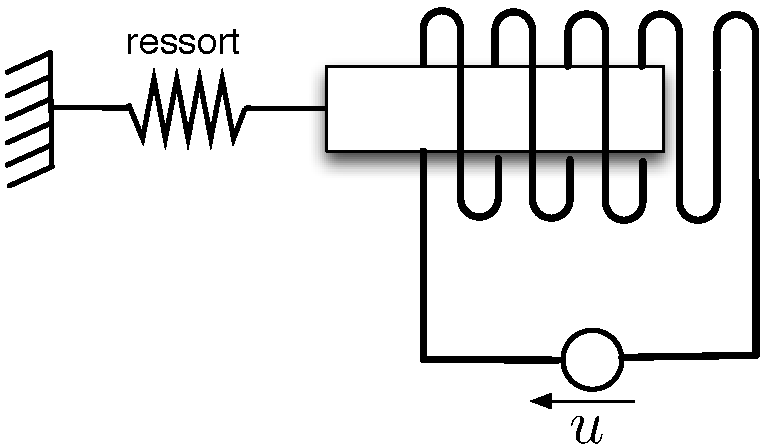
\includegraphics[height=3cm]{convem}
\caption{electromechanical converter}
\label{fig:convem}
\end{center}
\end{figure}

Suggest a state-spaced model of this system according to the following  modeling assumptions :
\begin{enumerate}
\item The core movement is forced to be linear by a slide.  The friction can be considered as viscous and linear.
\item The core is shorter than the solenoid.
\item The flow in the solenoid is a linear function of the length $h$ of the core part which is inside the solenoid.
\item The flow is a saturated monotonically increasing function of the current.
\item The spring is linear. \qed
\end{enumerate}
\end{exercice}

\begin{exercice}{\bf \em Clockwork motor}
A small motor used in watchmaking is presented in figure
\ref{fig:mothor}.  The stator is provided with field winding whose inductance
$L(\theta)$ is a sinusoidal function of the rotor angular position $\theta$.
\begin{figure}[htbp]
\begin{center}
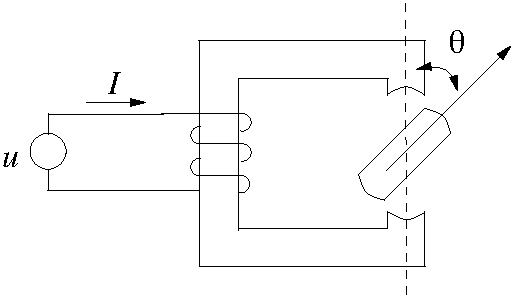
\includegraphics[height=40mm]{mothor}
\caption{Clockwork motor}
\label{fig:mothor}
\end{center}
\end{figure}
\begin{enumerate}
\item Suggest a model for the function $L(\theta)$ and compute the flow.
\item Establish the state-spaced model of the system assuming a linear viscous friction. The inputs are the 
voltage $u$ at the terminals of the inductor and the load torque $T_a$.
\item What has to be the waveform of the input signal $u$ when $T_a$ is constant and so that the rotor rotates at 
constant speed ?  \qed
\end{enumerate}
\end{exercice}
\newpage

%%%%%%%%%%%%%%%%%%%%%%%%%%%%%%%%%%%%%%%%%%%%%%%%%%
%%%%%%%%%%%%%%%%%%%%%%%%%%%%%%%%%%%%%%%%%%%%%%%%%%
%%%%%%%%%%%%%%%%%%%%%%%%%%%%%%%%%%%%%%%%%%%%%%%%%%
%%%%%%% PARTIE DE Nicolas Stevens    %%%%%%%%%%%%%%
%%%%%%%%%%%%%%%%%%%%%%%%%%%%%%%%%%%%%%%%%%%%%%%%%%
%%%%%%%%%%%%%%%%%%%%%%%%%%%%%%%%%%%%%%%%%%%%%%%%%%
%%%%%%%%%%%%%%%%%%%%%%%%%%%%%%%%%%%%%%%%%%%%%%%%%%

\begin{exercice}{\bf \em Unipolar off-phase synchronous machine} %Machine synchrone unipolaire diphasée.

This is a machine holding two stator windings (labelled $a$ and $b$) 
arrange in quadrature and a rotor winding (labelled $r$). 
The self and mutual inductances of the stator windings vary depending
on the angular position $\theta$ of the rotor according to the following laws : 
\eqnn 
L_a &=& L_o + L_1\cos 2\theta \nonumber \\ 
L_b &=& L_o - L_1\cos 2\theta \nonumber \\ 
L_{ab} &=& L_1 \sin 2\theta \nonumber 
\eeqnn 
The self inductance of the rotor $L_r$ is constant. The mutual 
inductances between the rotor and the stator windings are expressed in
terms of $\theta$ : 
\eqnn 
L_{ar} &=& L_2 \cos \theta \nonumber \\
L_{br} &=& L_2 \sin \theta \nonumber  
\eeqnn
\begin{enumerate} 
\item Establish the coupling equations of the electromechanics 
system (see Section 3.4) 
\item The rotor is supplied by a constant current source
$I_r$. Establish the state model of this machine when 
it works as a motor (you might need to use the example 3.3). \qed
\end{enumerate}
\end{exercice}
\vv

\begin{exercice}{\bf \em Elementary machine with two windings.}

Let's consider the elementary machine with two windings working as 
a generator, such as it is described in the example 3.3.
Denote how to revise the state equations under the following hypothesis : 
\begin{enumerate}
\item  The electric charge of the stator circuit is capacitive
\item  The rotor winding is closed using a short-circuit. \qed
\end{enumerate}
\end{exercice}
\vv

\begin{exercice}{\bf \em DC motor with self-excitation}

A DC motor with self-excitation is designed such as the stator 
current and the rotor current are supplied by the same power source
(see figure \ref{fig:autoex}). Establish the state model
of this system using the tension source $u$ as the only input 
variable of this system. \qed
\begin{figure}[htbp]
\begin{center}
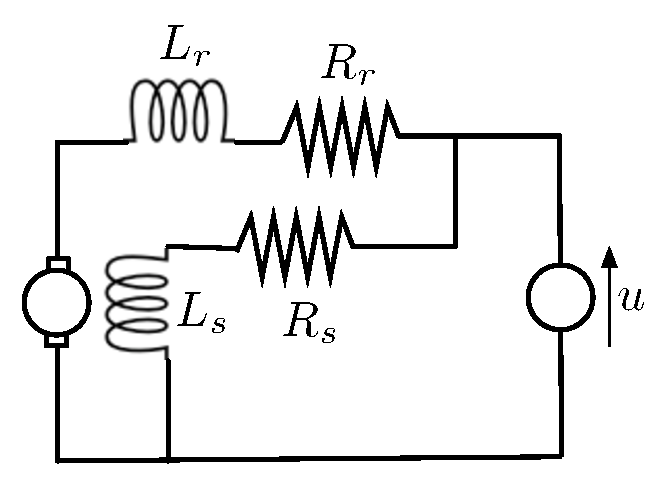
\includegraphics[height=4cm]{autoex}
\caption{DC motor with self-excitation}
\label{fig:autoex}
\end{center}
\end{figure}
\end{exercice}
\vv

\begin{exercice}{\bf \em DC generator with self-excitation}
Let's consider a DC generator with self-excitation. The rotor tension 
induced at constant rate is a {\em strictly increasing and bounded} function 
depending on the excitation current $E(I_s)$ such as $E(0) >
0$. The generator provides a capacitive electric charge. 
The input control variable of the system is the angular velocity of 
the generator. 
\begin{enumerate}
\item Propose an analytical form for the function $E(I_s)$.
\item Propose a state model for this system.
\item Justify the existence of a non-zero residual voltage $E(0)$. \qed
\end{enumerate}
\end{exercice}
\vv

\begin{exercice}{\bf \em DC motor with off-center load}

A DC motor with independent excitations and controlled by the rotor current
drives an off-center load (the motor shaft do not pass through the 
center of mass of the load : indeed, there is an unbalanced effect)
through a transmission whose flexibility is significant. 
Propose a state model taking into account this features. 
\end{exercice}
\vv

\begin{exercice}{\bf \em DC-DC converters}

\begin{figure}[htbp]
\begin{center}
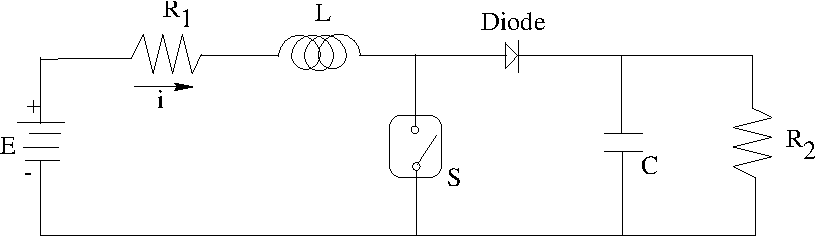
\includegraphics[width=85mm]{DCDC}
\caption{DC-DC converter}
\label{fig:DCDC}
\end{center}
\end{figure}
The circuit depicted at the figure above describes a DC-DC converter.  
The device labelled "S" pictures an electronic switch of type MOSFET 
which is open and close periodically.\\

Establish a state model of the system under the following modelling 
hypothesis :
\begin{itemize}
\item[a)] the voltage $E$ of the supply battery is constant
\item[b)] both resistances $R_1, R_2$, the inductance $L$ and the 
capacitor $C$ are linear
\item[c)] the input variable is the commutation frequency of the switch. \qed
\end{itemize} 
\end{exercice}



\end{document}
